% !TEX root = 99_main.tex

The experiment, consisting of fifteen users each equipped with a Fitbit over a month, produced a data set of 1,460 data points. Each data point is effectively a survey of the user at a particular time. The results presented in this section is a demonstration of the type of analysis that can be conducted using data acquired from the \emph{cozie} clock-face.

\subsection{Overview of spatio-temporal data}
Figure \ref{fig:summary}a details the spatial distribution of data throughout Singapore. Each of these data points is tagged with the users heart-rate, response, and local temperature which can be used to infer faults or issues within the building. Figure \ref{fig:summary}b is a simple heat map plotting the number of responses based on the hour of the day, and day of the week. It is interesting to note that 55\% of responses come from the hours of 9:00, 11:00, 13:00, 15:00, and 17:00 when the occupant is buzzed and forced to give feedback. The remaining 45\% of responses are made outside these times through the self-motivation of the participants themselves. Figure \ref{fig:summary}c details the daily responses from the participants, and no observable decrease in responses can be made, indicating no effects of survey fatigue. Dips in responses naturally occur during the weekend, and during the first week when users were still being onboarded. A normal distribution of heart-rate data from the Fitbit heart rate sensor can be found in Figure \ref{fig:summary}d.

\subsection{Merging with environmental sensor data}
Combining the cozie clock-face, with additional environmental sensors opens further dimensions of analysis. User responses are mapped to the environmental condition at which they are exposed, which can provide a high quality labelled data set for training data-driven models. Figure \ref{fig:summary}e-f detail the distribution of temperature and humidity data. Unfortunately, due to communication issues from these sensors, not all data points could be recorded. The temperature of the strap-mounted temperature sensor is on average 0.8 $^\circ$C warmer than the surrounding environment due to the influence of body temperature. 

\begin{figure}
\begin{center}
\includegraphics[width=\textwidth, trim= 0cm 0cm 0cm 0cm,clip]{cozie_datasummary.pdf}
\caption{Overview of raw data extracted from the cozie clock-face and additional sensors. (a) spatial distribution of responses throughout Singapore, (b) temporal distribution of responses, (c) number of responses per day over the course of the experiment, (d-f) rug plots detailing the normalised distribution of responses based on the Fitbit heart rate sensor, wrist-mounted temperature sensor, and off-body humidity sensor }
\label{fig:summary}
\end{center}
\end{figure}



\subsection{Clustering of thermal comfort personality}
\label{ch:userResults}
Individual user feedback can be clustered using unsupervised learning techniques. In this example, we use a hierarchical k-means clustering based on Euclidean distance using the nearest-point-algorithm. The results, shown in Figure \ref{fig:clustering}, show four distinct clusters of users. 

Understanding and defining these differences in user preferences can be used to recommend spaces that may better suit the needs of the occupant. For example, Group A, which primarily works off-site can be recommended alternative workspaces that are on average cooler. Group C on the other hand is a single highly satisfied user, who works from a single work-space within a narrow temperature range, and relatively low resting heart-rate. Group D represents our conventional occupant that may be comfortable 70\% of the time. 

Below the cluster plot are spatial distributions of responses that can be used to identify different building climates. The majority of \emph{Prefer Warmer} responses occur in co-working space 1. This area can be labelled as a \emph{cooler working space} for users that would prefer cooler working environments. Alternatively, if facilities management wishes to save energy, increasing the set-point temperature of these \emph{over-cooled} spaces may be a low effort solution which may simultaneously improve occupant well-being. 



\begin{figure}
\begin{center}
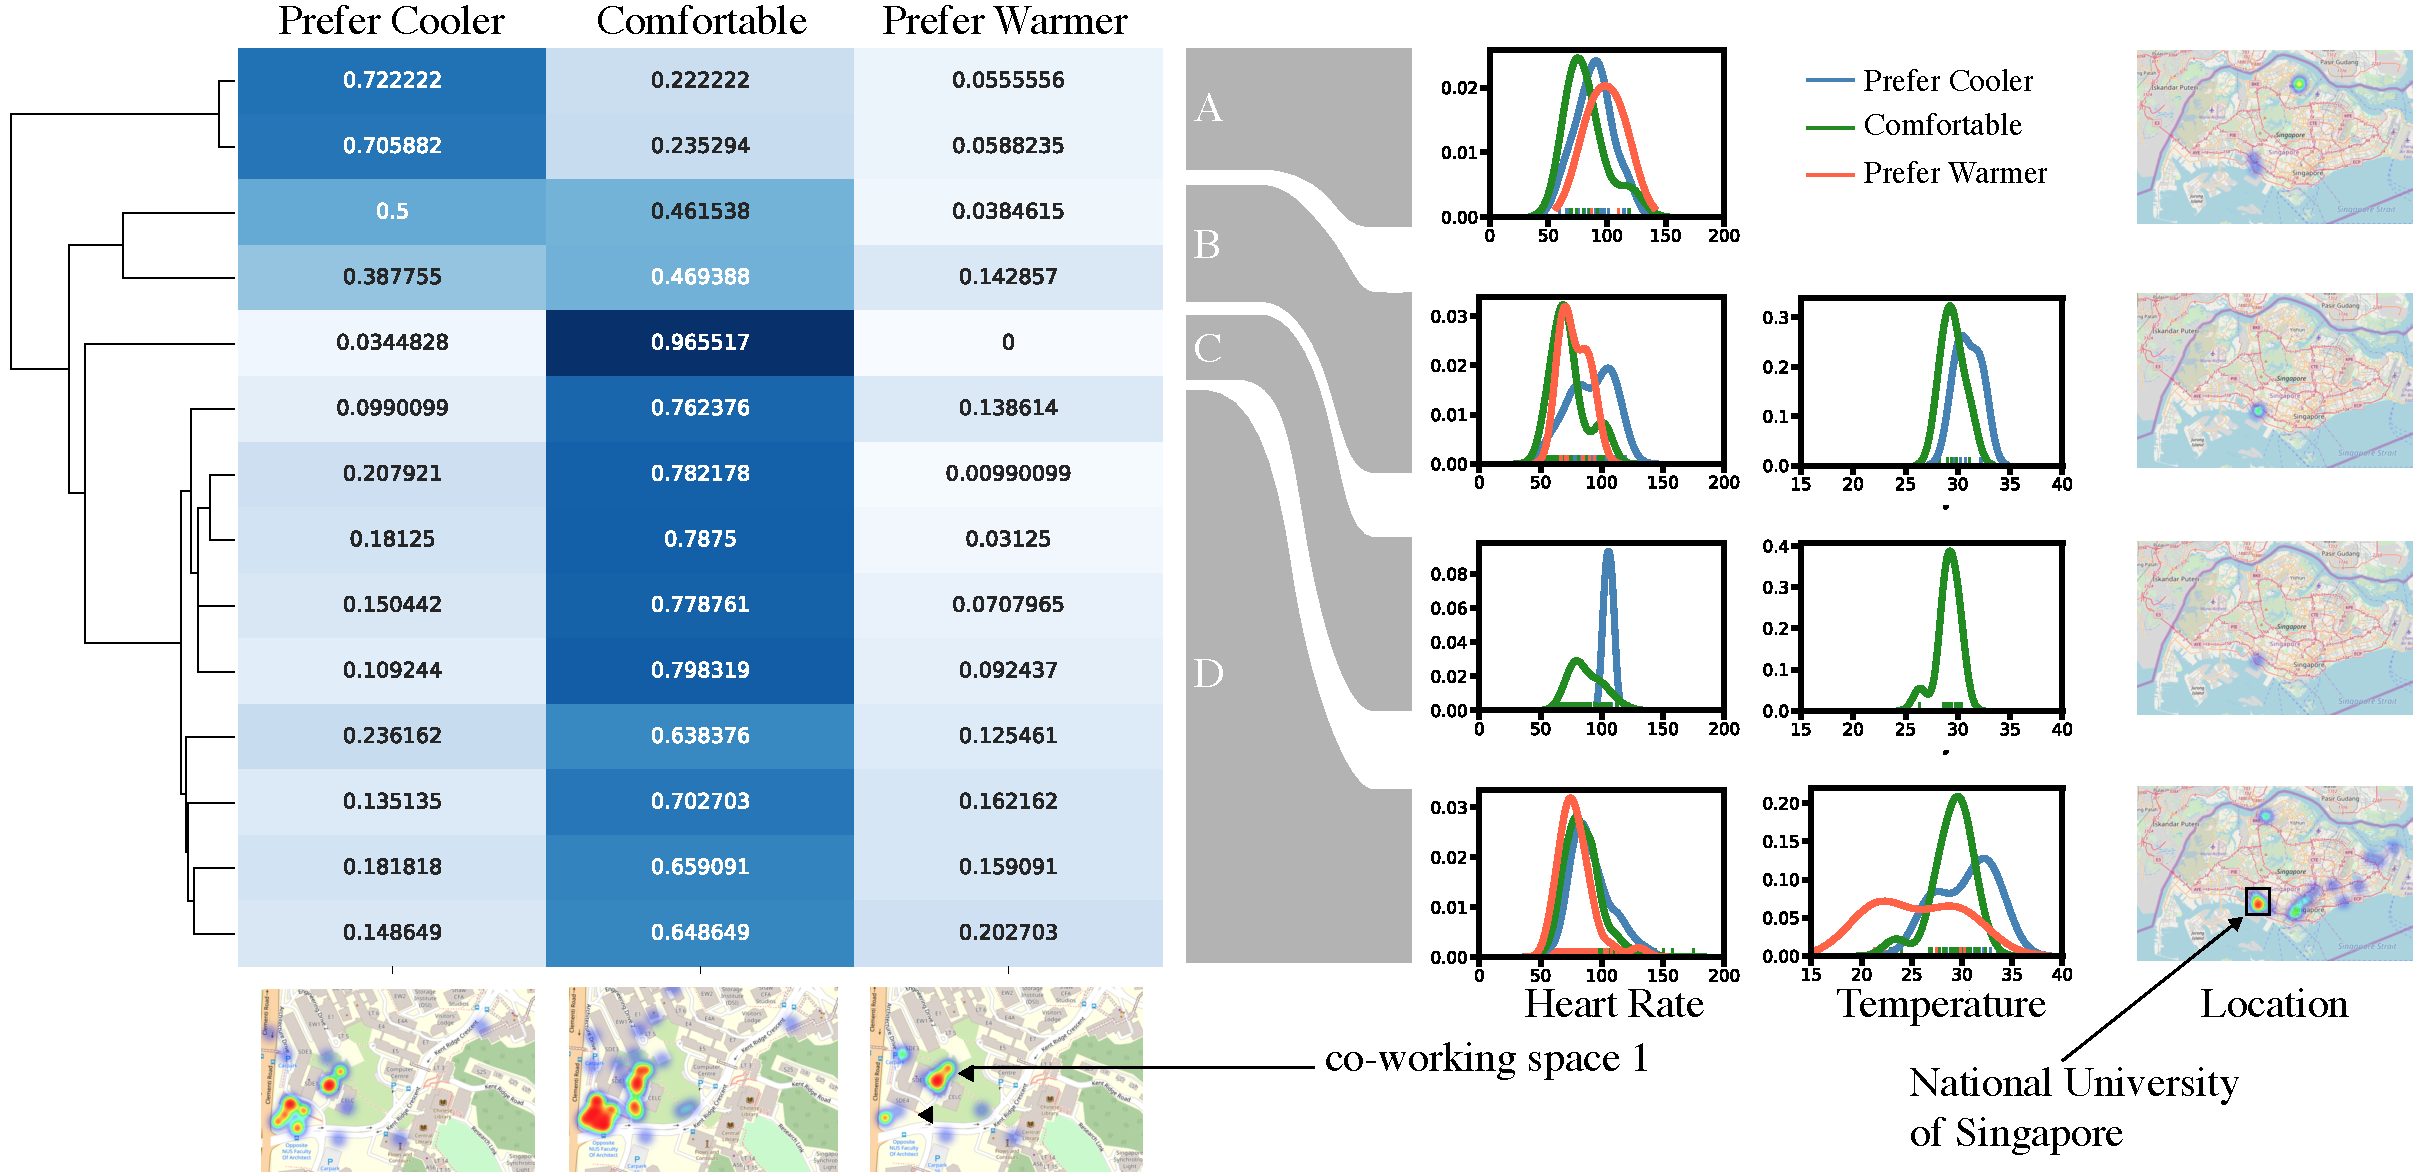
\includegraphics[width=\textwidth, trim= 0cm 0cm 0cm 0cm,clip]{cluster_results_compressed.pdf}
\caption{Hierarchical clustering heatmap of user feedback using k-means with Euclidean distance. The numbers within the cluster-map detail the normalised number of responses. Four distinct groups can be observed. (A) two users that generally prefer cooler environments to their norm, (B) users that are comfortable 50\% of the time, (C) user that is almost always comfortable, (D) users that are comfortable on average 70\% of the time. To the right are breakdowns of the respective groups via sensor data and location. Below the cluster plot are spatial distributions of feedback responses at the university.}
\label{fig:clustering}
\end{center}
\end{figure}


